\section{Novel Limiting Criterion and Limiting Process}\label{limSec}

Like other high-order methods, DGFEM needs to be limited around the shocks to avoid instability of the scheme.

In case of solution described by the first order polynomials (i.e. linear functions), the limiting method can be done by global limiting process and minmod limiter can be used to decide if the solution should be limited. However, this method cannot be used in case of the second order polynomials as the slope of the solution cannot be easily compared by the upwind and downwind differences
\begin{equation}\label{diff}
\delta^- W_{i,k}=\frac{W_{i,k}-W_{i-1,k}}{\Delta x},\quad \delta^+W_{i,k}=\frac{W_{i+1,k}-W_{i,k}}{\Delta x},
\end{equation}
which are used in minmod limiter. Here $\Delta x$ means the distance between the middles of the adjacent finite volumes.

The initial conditions of the classical Riemann problem can bee seen in Figure \ref{riemann} where the water depth and flat bed function is plotted. The initial velocity is zero.
\begin{figure}
\centering
\includegraphics[width=0.7\textwidth]{OBR/riemann.eps}
\caption{Initial conditions of the Riemann problem.}\label{riemann}
\end{figure}
\begin{figure}
\centering
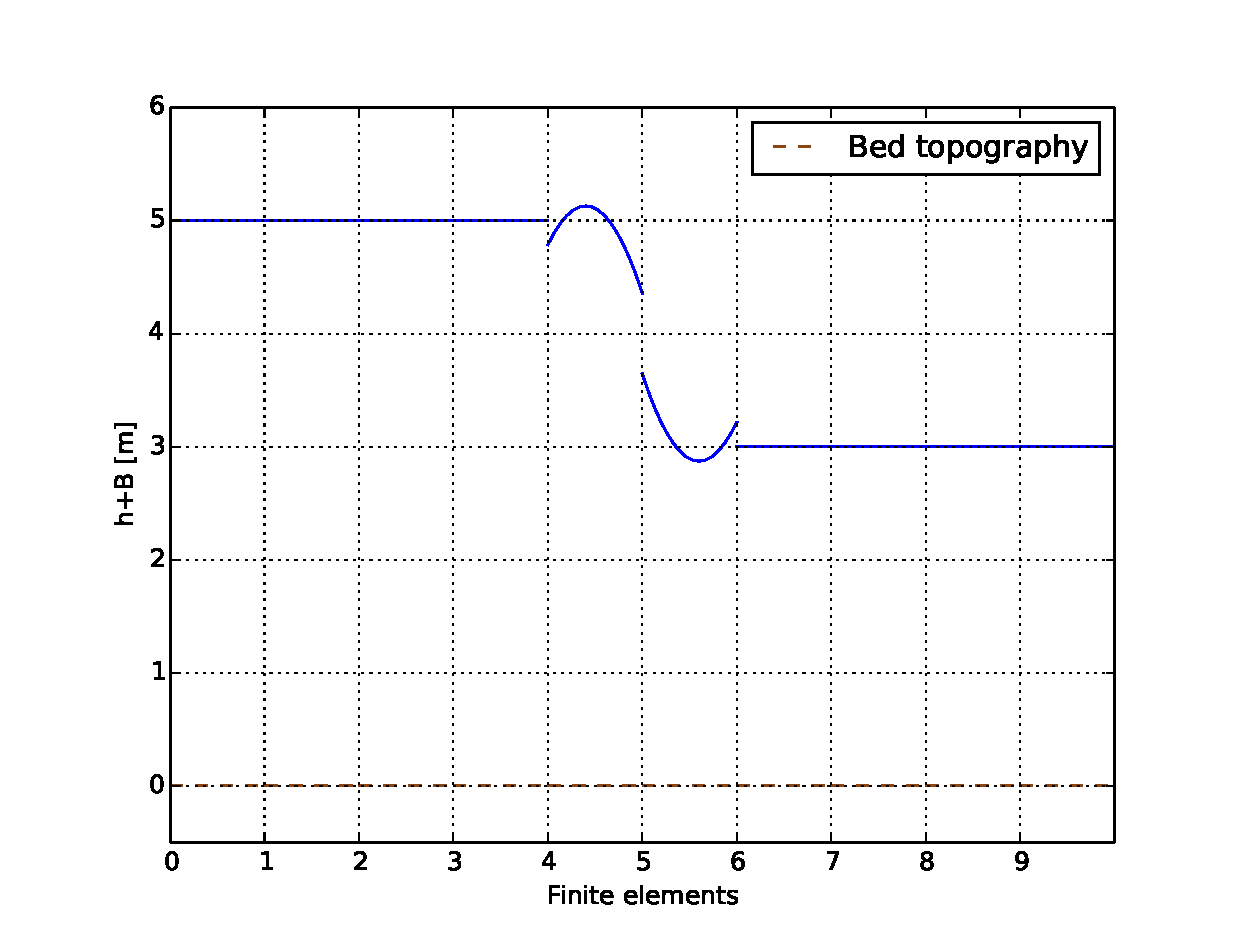
\includegraphics[width=0.7\textwidth]{OBR/first.eps}
\caption{First time iteration of non-limited water depth.}\label{first}
\end{figure}
\begin{figure}
\centering
\includegraphics[width=0.7\textwidth]{OBR/HU.eps}
\caption{First time iteration of non-limited discharge.}\label{HU}
\end{figure}
It is very likely that non-limited solution around the shock is not monotone and concave or convex as shown for water depth and discharge in Figures \ref{first} and \ref{HU}. The novel criterion for the second order polynomial base functions suppose, that the solution in the centre of the finite element must be bounded by the values at the edge of this element. If the solution in the middle is not bounded, i.e.
\begin{equation}\label{crit}
\begin{array}{c}
 min\left(W_{i,k}(x_{i-\frac12},t),W_{i,k}(x_{i+\frac12},t\right)>W_{i,k}(x_i,t)\\
\text{or}\\
 max\left(W_{i,k}(x_{i-\frac12},t),W_{i,k}(x_{i+\frac12},t)\right)< W_{i,k}(x_i,t)
 \end{array}
\end{equation}
the cell is defined as 'troubled' and the solution of a conservative variable must be limited in this cell.

The solution in the 'troubled' cells must be limited. The limiting process, used within this work, is similar to the limiting process of Cockburn and Shu \cite{Cockburn1989b}. This process consist in lowering the polynomial order and employing suitable limiter. As a basis functions the Legendre polynomials are used.

 This polynomials can bee seen in Table \ref{table:legendre}.
\begin{table}
\caption{Legendre polynomials}
\centering
\begin{tabular}{|c|c |}
\hline
Base function & Legendre polynomial\\
\hline
\hline
$\varphi^1$ & 1\\
$\varphi^2$ & x\\
$\varphi^3$ & $\frac12\left(3x^2-1\right)$\\
\hline
\end{tabular}
\label{table:legendre}% is used to refer this table in the text
\end{table}
Let us consider the range of these polynomials $[-1,1]$. Interval $[-1,1]$ can be mapped to the arbitrary interval $[x_{i-\frac12},x_{i+\frac12}]$ by linear transformation (linear mapping)
\begin{equation}\label{mapping}
x=x_{i-\frac12}\frac{1-\xi}{2}+x_{i+\frac12}\frac{1+\xi}{2}, \quad x\in[x_{i-\frac12},x_{i+\frac12}],
\quad \xi\in[-1,1].
\end{equation}

  Legendre polynomials are orthogonal in 'integral average' norm, i.e.
\begin{equation}
\int_{-1}^{1} \varphi^j \varphi^l dx \begin{cases}
=0 \text{ for }i\neq j\\
\neq 0 \text{ for }i=j\\
\end{cases}
\end{equation}
thus the integral averages of $\varphi^2$ and $\varphi^3$ are zero\footnote{The integral averages of higher Legendre functions are zero because of the orthogonality with the first one $\int_{-1}^{1} \varphi^{j}\cdot \underbrace{1}\limits_{\varphi^{1}} \ dx=0, \ j=2,3$.} itself and the scheme is still mass and momentum conservative even if the third coefficient $w_{i,k}^{3}$ from (\ref{linC}) is set to be zero.


 Within this work, the minmod limited was chosen to modify the second coefficient
\begin{equation}\label{clasLim}
w_{i,k}^{2}=minmod(\delta^- W_{i,k},\delta^+ W_{i,k})
\end{equation}
where upwind and downwind differences $\delta^\mp W_{i,k}$ are defined by (\ref{diff}) and $minmod$ function is defined as \cite{Nessyahu}
\begin{equation}\label{limiter}
\text{minmod}(z_1,z_2)=\frac{1}{2}[\text{sgn}(z_1) + \text{sgn}(z_2)] \cdot \text{min}(|z_1|, |z_2|).
\end{equation}

\subsection{Implementation of the Surface Gradient Method}
In \cite{Zhou2001}, the Surface Gradient Method (SGM) was introduced. This method has been developed for reconstruction of the water level within the shallow water equations with bed slope source terms. In contrast
to conventional data reconstruction methods based on water depth ($h$) the
water surface level ($h+B$) is chosen as the basis for data reconstruction. This provides
accurate values of the conservative variables at cell interfaces so that the fluxes can
be accurately calculated with a Riemann solver.

If the SGS method is adopted, the 'troubled' cell criterion (\ref{crit}) is defined as
\begin{equation}\label{critH}
\begin{array}{c}
 min\left(W_{i,1}(x_{i-\frac12},t)+B(x_{i-\frac12}),W_{i,1}(x_{i+\frac12},t)+B(x_{i+\frac12})\right)>W_{i,1}(x_i,t)+B(x_i)\\
\text{or}\\
 max\left(W_{i,1}(x_{i-\frac12},t)+B(x_{i-\frac12}),W_{i,1}(x_{i+\frac12},t)+B(x_{i+\frac12})\right)< W_{i,1}(x_i,t)+B(x_i)
 \end{array}
\end{equation}
The limiting process is similar to the process described earlier. The third coefficient $w_{i,1}^{3}$ is set to zero. The difference is in computation of the second coefficient $w_{i,1}^{2}$. Upwind and downwind differences used in the limiter (\ref{limiter}) are computed as
\begin{equation}\label{diffH}
\delta^- W_{i,1}=\frac{\left(W_{i,1}+B_{i}\right) - \left(W_{i-1,1}+B_{i-1} \right)}{\Delta x},\quad \delta^+W_{i,1}=\frac{\left(W_{i+1,1}+B_{i+1}\right) - \left(W_{i,1}+B_{i} \right)}{\Delta x}.
\end{equation}
As in the vector of the conservative variable (\ref{konz}), the water depth (instead of the water level) is stored, the second coefficient must be computed as
\begin{equation}
w_{i,1}^{2}=minmod(\delta^- W_{i,1},\delta^+ W_{i,1})-\delta B_i
\end{equation}
where $\delta B_i$ means the slope of the bed function computed as
\begin{equation}
\delta B_i=\frac{B_{i+\frac12}-B_{i-\frac12}}{\Delta x_i}.
\end{equation}
 Provided that the piece-wise linear bed function is also described by the linear combination of the bed function coefficients $w_{i}^j$ and the first two Legendre polynomials
\begin{equation}
 B_i(x)=w_{b_{i}}^1 \cdot 1+w_{b_{i}}^2 \cdot x,
 \end{equation}
 $\delta B_i$ is identical to the coefficient $w_{i}^2$. Index $b$ implicates that the $w_{b_{i}}$ coefficients belong to the description of the bed function.
